\chapter{Instrumentation} \label{chp:instrumentation}
\section{Introduction} \label{sec:instrumentation/introduction}
Flexible and efficient instrumentation is the foundation of this project. Here, possible approaches to this instrumentation are discussed, along with critical analyses.

There are two main approaches to the instrumentation: automatic, and manual. 

\section{Automatic Approaches} \label{sec:instrumentation/automatic}
	In this context, an automatic approach to instrumentation is a technique that can be applied directly at compile-time (or just before run-time in an agent-like fashion). Such approaches require no human intervention whatsoever, and have the additional advantage of having access to additional compile-time meta-data which is not possible to gain at run-time or using manual instrumentation.

	\subsection{Graal} \label{sec:instrumentation/graal}
	In the first instance, an automatic approach based on Graal was investigated. Graal was chosen in the first instance because it is the most flexible approach: it allows the combination of compile-time evaluation, as well as run-time evaluation of the dependency algorithms.
	
	As mentioned, Graal uses various different forms of intermediate representation, based on graphs (see section \ref{sec:graal/ir}). In principle, it should be possible to modify these graphs in order to invoke the instrumentation (described in chapter \ref{chp:runtime}).
	
	Modifying graphs in Graal is made easy through a simple API. A user can define custom phases (see section \ref{sec:graal/transformations}). Pseudocode for this is as follows:
	
	\begin{lstlisting}[caption=Sample code for adding a phase and manipulating a graph,label=list:graph-trans]
	// create the phase
	public class MyPhase extends Phase {
	    @Override
	    protected void run(StructuredGraph graph) {
	        // modify the graph
	        for (LoadIndexedNode node:
	            graph.getNodes(LoadIndexedNode.class)) {
	            graph.addAfterFixed(node,
	                graph.add(new MyCustomNode()));
	        }
	    }
	}
	
	// add the phase
	Suites s = Graal.getRequiredCapability(SuitesProvider.class)
	    .createSuites();
	s.getHighTier().appendPhase(new MyPhase());
	\end{lstlisting}
	
	The call to \texttt{getHighTier()} can be replaced with equivalent methods for the other IRs (\ie, \texttt{getLowTier()} and \texttt{getMidTier()}.
	
	As we can see in figure \ref{fig:access-index}, which displays the high-level graph for a simple method that takes an array actual parameter and returns index $0$ of that array, there are specialised nodes for array accesses: \texttt{LoadIndexedNode}. Note that there is also an equivalent for array store operations, \texttt{StoreIndexedNode}.
	
	\begin{figure}[h]
		\centering
		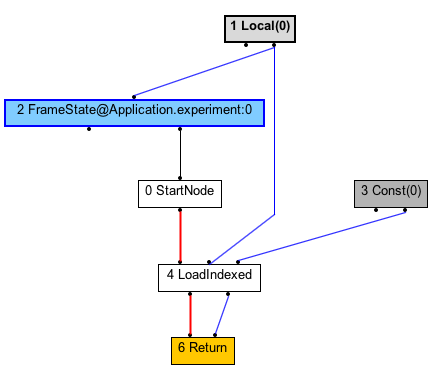
\includegraphics[width=.7\textwidth]{graphics/access-index.png}
		\caption{A high-level graph (with inlining disabled) for a simple method taking an array actual parameter, returning index 0}
		\label{fig:access-index}
	\end{figure}
	
	This is the basis for selecting the appropriate nodes to instrument. One additional advantage of Graal is the richness of the information available at compile-time. Figure \ref{fig:graal-meta} shows all the available information, as seen in Eclipse's debugger.
	
	\begin{figure}[h]
		\centering
		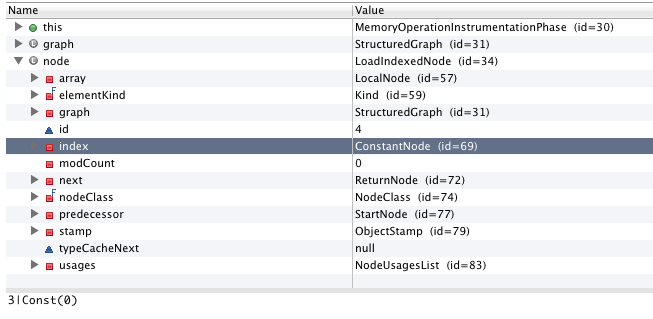
\includegraphics[width=0.8\textwidth]{graphics/graal-metadata.png}
		\caption{Information available at compile-time for the \texttt{LoadIndexedNode} shown in figure \ref{fig:access-index}}
		\label{fig:graal-meta}
	\end{figure}
	
	The availability of predecessor and next nodes, as well as nodes representing indexes (in this case, a \texttt{ConstantNode}) highlights another advantage of using Graal for these transformations - static analysis is possible, which means that instrumentation can be disabled if dependencies can be proven statically. 
	
	There are several possibilities for adding instrumentation in Graal.
	
	\begin{enumerate}
		\item \label{item:instr1} Add a custom node type, which is lowered to an invoke instruction after each applicable node.
	
		\item \label{item:instr2} Replace the nodes in question with a custom node that implements the same operation in addition to the required behaviour.
	
		\item \label{item:instr3} Javassist includes a method for replacing all array accesses with method calls \citep{JavassistDocs}. It may be possible to use Graal to replace the method call targets where instrumentation is required. In cases where no instrumentation is required, the method would return the array value (or perform the store), which would then be inlined by the compiler.
	\end{enumerate}
	
	In cases \ref{item:instr1} and \ref{item:instr2}, then node would need to implement \texttt{Lowerable}, an interface in Graal that allows nodes to be lowered between IR levels.
	
	\textit{However}, there is currently a limitation in Graal which means that it is not currently possible to insert calls to (static) methods. This is because there is no \emph{bytecode index} (or BCI) for the interpreter to return to if a deoptimisation occurs (details on Graal's deoptimisation mechanisms are available in section \ref{sec:graal/deopt}). Since methods calls cannot be guaranteed to be deoptimisation-free, they cannot be inserted into graphs. Any static methods that modify abstract data types (\ie, the storage formats described in section \ref{sec:runtime/storage}) cannot be assumed to be deoptimisation free. Modifying a data structure violates the optimisation assumptions, causing a deoptimisation. The interpreter then tries to resume from the BCI of the invoke. However, there is no BCI associated with inserted invocation, meaning that the interpreter cannot resume in the event of the inevitable deoptimisation. The end result is that insertation of arbitrary behaviour through invoke nodes to static methods is not currently possible in the Graal system.
	
	To illustrate the concept of BCIs, consider the following example. In Java bytecode, each instruction has an associated index (this example was compiled using \texttt{javap -c} from a basic `hello, world!' application):
	
	\begin{verbatim}
	Compiled from "Hello.java"
	public class Hello {
	  public Hello();
	    Code:
	       0: aload_0       
	       1: invokespecial #1    // Method java/lang/Object."<init>":()V
	       4: return        
	
	  public static void main(java.lang.String[]);
	    Code:
	       0: getstatic     #2    // Field java/lang/System.out:Ljava/io/PrintStream;
	       3: ldc           #3    // String Hello, world
	       5: invokevirtual #4    // Method java/io/PrintStream.println:(Ljava/lang/String;)V
	       8: return        
	}
	
	\end{verbatim}
	
	We can clearly see the BCIs of the various operations: the \texttt{invokespecial \#1} has a BCI of 1, and so on.

	This is a limitation of the Graal platform. In the coming months, the Graal core developers are adding this required feature. Once the feature has been added, it is a simple modification (as the infrastructure has already been created) to add this into Graal. Indeed, the required infrastructure for this transformation has been created -- once the support for it is available, only would need to enable the transformations.
	
	As an alternative, we used manual instrumentation (section \ref{sec:instrumentation/manual}). Although this does have the disadvantage of requiring both source-code access as well as human effort, this will not affect the results or correctness of the evaluation as the semantics are equivalent. The results and conclusions of this report will not be affected by this shortcoming of Graal. The required framework and infrastructure has already been developed, the mechanism through which the framework is used cannot affect the results in this case.
	
	The remaining sections of this chapter consider possible alternative approaches to automatic instrumentation. 

	\subsection{Bytecode Instrumentation} \label{sec:instrumentation/bytecode-instr}
	The first approach uses so-called \textit{bytecode instrumentation} (BCI) - that is, modifying the bytecode directly, either at compile-time or runtime. This approach is advantageous in that arbitrary commands can be inserted, and is only subject to the limitations of the bytecode format. In this sense, arbitrary functionality can be inserted into \texttt{.class} files. However, it is complex (requiring advanced knowledge of the JVM and bytecode formats), as well as being difficult to use. Graal already performs a lot of the work that would be required with this kind of approach, in that it detects control flow and memory dependencies from bytecode. Such systems require a large degree of programmer effort.

		\subsubsection{Java Agents} \label{sec:instrumentation/bytecode-instr/agents}
		At the heart of BCI is the idea of Java Agents \citep{javaagents}. In order to understand them, however, one must first understand some details of the Java platform.
		
		Unlike some other languages (for example, C and C++\footnote{Although note that C and C++ \emph{also} support dynamic linking}), Java is a dynamically linked language. That is to say that the various different libraries (JARs) that Java programs used are linked at run-time, rather than compile-time. The advantage to this approach is that it allows distributables to be smaller in size (recall Java Network Launching Protocol, a method for launching (and therefore, distributing) Java applications over the Internet). The disadvantage to this approach is that it can lead to `dependency hell', although through the combination of versioning metadata in JARs and the extreme backwards compatability mantra in Java, this is not currently a significant issue.
		
		There are three main class loaders in Java:
		
		\begin{itemize}
			\item The system class loader loads the classes found in the \texttt{java.lang} package
			\item Any extensions to Java are loaded via the extension loader
			\item JARs found within the class path are loaded with the lowest precedence, these include the majority of user-level libraries
		\end{itemize}
		
		Java Agents manipulate class files at load-time, through the \texttt{java.lang.instrument} package. The package defines the \texttt{ClassFileTransformer} interface, which provides implementations of class transformers. An advantage of this approach is that since Java Agents are included in the core Java package, developers wishing to use \textit{Locomotion} would not need to download and install Graal.
		
		There are several different libraries which provide an abstraction layer for such bytecode transformations. The following sections describe various different libraries that could be used (or use themselves) for agent-based bytecode instrumentation.

		\subsubsection{ASM} \label{sec:instrumentation/bytecode-instr/asm}
		Despite Java Agents providing the capability to manipulate raw Java bytecode (indeed, the bytecode is made available as a \texttt{byte} array), performing such transformations are difficult and awkward. For this reason, there exists many different libraries for manipulating Java bytecode, ObjectWeb ASM being one of them.
		
		ASM \citep{Bruneton2002} is a simple-to-use bytecode manipulation library, itself written in Java. It uses a high-level abstraction for the bytecode, which is advantageous because it allows developers to remain unconcerned with the specifics of control flow analysis, dependency analysis and other such concerns.
		
		Although now common, when ASM was first developed it was considered particularly innovative because it allowed the use of the visitor pattern \citep[p.~331]{Gamma1995} for traversing bytecode. The visitor pattern `allows for one or more operations to be applied to a set of objects at runtime, decoupling the operations from the object structure' \citep{McDonald2008}. The advantage to this approach is that it allows a user to walk a serialized object graph \emph{without} de-serialising it or defining large numbers of classes (for reference, an alternative to ASM for bytecode generation, BECL \citep{ApacheBECL} contains 270 classes for representing each bytecode). Additionally, it allows users to also reconstruct a modified version of the graph (in ASM, graphs are immutable).
		
		Several well-known existing projects use ASM already for bytecode generation, including the Groovy programming language \citep{GroovyDocs}. I also have some experience of ASM through the \textit{Compiling Techniques} coursework \citep{CTcoursework}.
		
		ASM was selected as a possible alternative for this project for several reasons. Firstly, its visitor pattern-based approach to bytecode generation/modification is high-level and easily understandable. It also has high performance, being a factor of 12 more performance than BECL for serialisation/deserialisation, and a factor of 35 times more performance than BECL for computing maximum stack frame sizes. ASM is also superior to BECL for performing modifications, although with a significantly lower margin of just a factor of four.
		
		The reason for this performance improvement is likely the way ASM and BECL are designed. BECL follows a strict, classical interpretation of object-oriented design principles. Although `good' software design, it is well known that object models have considerable overhead.

		\subsubsection{Javassist} \label{sec:instrumentation/alt-instr/bytecode-instr/javassist}
		Javassist \citep{Chiba1998} is similar to ASM in that it is also a library for manipulating bytecode, but its method of operation is significantly different. It allows for run-time polymorphism, by dynamically switching implementation of classes at run-time.
	
		There are also additional libraries for manipulating Java bytecode, but due to their features (or lack of), they were not considered for this project.

	\subsection{Aspect-Oriented Programming} \label{sec:instrumentation/alt-instr/aop}
	Aspect-Oriented Programming (AOP) \citep{Kiczales1997} is another dialect of object-oriented programming that aims to significantly increase separation of concern within programs, so that programs are more loosely coupled. AOP is a direct descendent from object-oriented programming as well as reflection. Reflection allows programmers to dynamically introspect classes at run-time; changing values and so on. AOP takes this to another level, by allowing so-called \textit{advice} to be specified (essentially the additional behaviour to be added) and added to \textit{join points}, which are arbitrary points of control flow within the program.
	
	When combined, aspect-oriented systems add these behaviours to the program in question at compile-time through a process called \textit{weaving}.
	
	To illustrate this concept, consider the problem of logging method calls. In traditional systems, at each function/method definition the programmer would need to add specific logging code:
	
	\begin{lstlisting}[caption=Traditional use of advice in programs,label=lst:tradadvice]
def function name(...) {
    if (DEBUG)
        println("function called at " + time());
      
    // other statements
}\end{lstlisting}
	
	This behaviour is called an \textit{aspect} (an area of a program which may be repeated several times which is unrelated to the purpose of the program). If the behaviour is to change (\eg for example, changing the call to \texttt{date()} to a call to \texttt{time()} instead), each method declaration must be changed manually - a time consuming and potentially error-prone task.
	
	Instead, the use of aspects allows the programmer to remove this functionality, and combine a pointcut and advice into an \textit{aspect}:
	
	\begin{lstlisting}[caption=AOP-based advice equivalent to listing \ref{lst:tradadvice},label=lst:aopadvice]
def aspect TraceMethods {
    def pointcut method-call: execution.in(*)
        and not(flow.in(this));
		
    before method-call {
        println("function called at " + time());
    }
}\end{lstlisting}
	
	Although that from a software engineering perspective this is clearly a superior solution (decreases coupling, increases reuse, increases separation of concern), the use of aspects has not been widely adopted. There are several likely causes for this, such as:
	
	\begin{itemize}
		\item \textbf{Lack of education}: like the other models that we have seen in section \ref{sec:introduction/parallelist}, widespread adoption of new programming construct requires that the average programmer can understand the feature without in-depth education in the model. AOP is somewhat counter to intuitive definitions of imperative or procedural languages, which hampers their adoption.
		\item \textbf{Lack of language support}: no widely adopted programming language comes with AOP included, or with an AOP library included in the standard library. Standard licensing issues also apply to third-party additions (\eg GPLv2/3 differences).
		\item \textbf{Unclear flow control}: perhaps the single largest issue with AOP. As noted by \citet{Constantinides2004}, aspects introduce effectively unconditional branches into code, mimicking the use of \texttt{goto} which \citeauthor{Dijkstra1968} famously considered harmful \citep{Dijkstra1968}.
		\item \textbf{Unintended consequences}: defining aspects incorrectly can lead to incorrect (global) state, \eg renaming methods and so on. If a team of developers are unaware of each other's modifications at weave-time, there may unintended consequences and subtle (or substantial) bugs introduced.
	\end{itemize}
	
	\subsection{AspectJ/ABC} \label{sec:instrumentation/aop/aspectj}
	AspectJ \citep{Kiczales2001} is an extension to the Java language that adds aspect-oriented features. It is a project of the Eclipse Foundation (of Eclipse IDE fame). The usage of AOP within Java is a somewhat natural extension as aspects can be seen as the modularisation of behaviour (concerns) over several classes - and not to forget that AOP was originally developed as an extension to object-oriented languages.
		
		\subsubsection{Array and Loop Pointcuts} \label{sec:instrumentation/aop/aspectj/arrayloop}
		However, the limitations of the AspectJ join-point model are somewhat obvious for this project. To be specific, `vanilla' AspectJ cannot define point cuts for neither array accesses or loops - a combination of which would be required for this project. In addition, the vanilla AspectJ implementation is not particularly extensible, which means that defining new point-cuts is somewhat difficult.
		
		There is, however, an implementation of AspectJ which \emph{is} designed to be more extensible and compatible (mostly) with the original AspectJ implementation - abc, the AspectBench Compiler for AspectJ \citep{Allan2005}.
		
		Although abc itself does not include point-cuts for either array access or loops, there exists two projects which, if combined, could offer the required features for this project.
		
		LoopsAJ \citep{Harbulot2005} is an extension to abc that adds a loop join point. This is not a trivial addition - when loops are compiled, they are compiled to forms that loose loop semantics (and instead use \texttt{goto} instructions). There are several forms that a loop can take, and a significant proportion of \citeauthor{Harbulot2005}'s work is in the identification of loops from the bytecode.
				
		For array access, the ArrayPT project \citep{Chen2007} adds additional array access capabilities to abc. Although the included point cut does include array access, it is somewhat limited and cannot determine either the index, nor the value to be stored. ArrayPT adds these capabilities to abc. ArrayPT defines two new point cuts, \texttt{arrayset(signature)} and \texttt{arrayget(signature)}. ArrayPT relies on the \texttt{invokevirtual} bytecode in the JVM.
		
		It is anticipated that, if these projects are combined, it would present a feasible approach to instrumentation.

	\subsection{Hybrid Models} \label{sec:instrumentation/hybrid}
		\subsubsection{DiSL} \label{sec:instrumentation/hybrid/disl}
		Recently, there has been renewed interest in Java bytecode instrumentation. Clearly, the use of aspect-oriented techniques is advantageous, but the current implementations (AspectJ/abc) are deeply flawed. In a sense, they are \textit{static} - they rely on predefined join and point-cuts before any aspect definitions can be constructed. DiSL is considered a hybrid approach because, unlike AspectJ which relies on access to source code, it uses an agents-based approach to aspect-oriented programming.
		
		DiSL (\textit{Domain Specific Language for Instrumentation}) \citep{Marek2012} is a new approach to a domain-specific language (which incidentally, implies that DiSL is declarative) for bytecode instrumentation. It does rely on the use of aspects, but it instead uses an open join-point model where any area of bytecode can be instrumented.
		
		\begin{itemize}
			\item Lower overheads
			\item Greater expressibility of aspect and join-point definition
			\item Greater code coverage
			\item Efficient synthetic local variables for data exchange between join-points
		\end{itemize}
		
		As opposed to AspectJ, which requires compile-time definition of join-points, DiSL uses an open-ended join point format which can be evaluated at weave-time. This allows arbitrary regions of bytecodes to be used as join points. \textit{Markers} are used to specify such bytecode regions (markers are included for common join points, such as method calls and, unusually, exception handling - a novel addition to aspect-systems in Java although control-flow analysis can be used to implement user-defined markers), while \textit{guards} allow users to further restrict selected join-points. Guards are essentially predicates which have access to only static information which can be evaluated at weave-time.
		
		DiSL implements advice in the form of \textit{code snippets}. Note the distinction between DiSL snippets and Graal snippets - although they are similar, DiSL snippets allow arbitrary behaviour to be inserted whilst Graal snippets are used to mainly lower complex bytecodes into simpler ones. Unlike other aspect-systems, DiSL does not support `around' advice. However, this is not usually regarded as a disadvantage per-se as synthetic local variables mitigate this.
		
		The semantics of snippets and guards is novel in DiSL. Both have complete access to local static (\ie, weave-time) reflective join-point information, meaning they can make (theoretically) unbounded numbers of references to static contexts. In addition, snippets have access to dynamic (\ie, run-time) information, including local variables and the operand stack.
		
		\citeauthor{Marek2012} present benchmarks of overheads with DiSL versus AspectJ, and their results are promising - a factor of three lower overheads, yet DiSL manages greater code coverage than AspectJ (the number of join-points captured is greater).
		
		In conclusion, DiSL represents a significant advancement in aspect-systems in general. DiSL allows many semantics of dynamically-typed languages to be expressed in the (statically-typed) Java language.
	
		\subsubsection{Turbo DiSL} \label{sec:instrumentation/hybrid/disl/turbo}
		An extension to DiSL, Turbo DiSL has been proposed by \citet[p.~353-368]{Furia2012}. Turbo DiSL is essentially an optimiser for DiSL which processes the bytecode produced by `vanilla' DiSL.
		
		There are several advantages of Turbo DiSL over DiSL. For example, instead of requiring expressions to be placed into separate classes, Turbo DiSL allows these expressions to be placed in the same class, increasing maintainability. Turbo DiSL also performs some standard compiler optimisations on DiSL-generated code, such as pattern-based code simplification, constant propagation and conditional reduction. These are supported by a novel partial evaluation algorithm.
		
		Turbo DiSL implements conditional reduction using partial evaluation. Many conditional control-flow statement expressions can be evaluated at weave-time -- Turbo DiSL removes these dead blocks. DiSL replaces these with \texttt{pop} commands\footnote{\url{http://homepages.inf.ed.ac.uk/kwxm/JVM/pop.html}}, resulting in program correctness remaining unchanged.
		
		In addition, an approach similar to peephole-based optimisation. For example, Turbo DiSL reduces unrequired instruction such as jumping to the next instruction, or optimising the conditional reduction effects. For each \texttt{pop} instruction found, the source bytecodes are found (i.e., which bytecodes push the to-be-popped operands). If those bytecodes are side-effect free, they both (the pop and the source) removed.
		
		The authors present an analysis of Turbo DiSL performance characteristics. The benchmarks selected were from the DaCapo benchmarks \citep{Blackburn2006}. There is a considerable increase in weave-time of a factor of 7.64 above the baseline, which clearly shows the drawbacks of partial evaluation. However, Turbo DiSL outperforms DiSL by a factor of 5.18 and 13 for startup and steady-state respectively - a considerable improvement.

		The authors present several uses cases where TurboDiSl is superior to DiSL (dynamic instrument configuration, tracking monitor ownership, field access analysis and execution trace profiling). However, this author speculates that, in spite of the aforementioned increase in weave-time, Turbo DiSL will completely supersede DiSL in all situations. 
		
\section{Manual Approaches} \label{sec:instrumentation/manual}
The major alternative to automatic instrumentation is manual instrumentation, where the user manually performs the required transformations in the source code.

These transformations consist of replacing array access and store operations with method calls, whilst adding relevant metadata if required. For example, consider the following array access:

\begin{lstlisting}[label=list:array-access,caption=Standard array access in Java]
int c = a[b];\end{lstlisting}

Manual instrumentation refers to replacing this operation, and all such operations, with the following (or equivalent):

\begin{lstlisting}[label=list:instrumented-array-access,caption=Instrumented array access]
int c = access-array(a, b);\end{lstlisting}

The \texttt{array-access} method (and the implied \texttt{array-store} method) performs the dependency checking algorithms using the techniques as described in section \ref{sec:runtime/analysis/online}.
	
\section{Summary} \label{sec:instrumentation/summary}
In this section, we have considered the use of Graal for automatic instrumentation. We have seen that, due to a limitation in the current version of Graal, it is not possible to add arbitrary static method invoke instructions. Regardless of this limitation, there are other possible approaches that could also (in principle) be used for automatic instrumentation.

Lastly, we have seen how manual instrumentation is possible, and the reasons why the alternative approach used (manual instrumentation) will not affect the results or conclusions of this dissertation.